\documentclass[a4paper, 11pt]{article}
\usepackage{mdframed}
\usepackage{comment} 
\usepackage{xparse}
\usepackage{tcolorbox}
\usepackage{lipsum} %This package just generates Lorem Ipsum filler text. 
\usepackage{fullpage} % changes the margin
\usepackage[a4paper, total={7in, 10in}]{geometry}
\usepackage[fleqn]{amsmath}
\usepackage{amssymb,amsthm}  % assumes amsmath package installed
\newtheorem{theorem}{Theorem}
\newtheorem{corollary}{Corollary}
\usepackage{graphicx}
\usepackage{tikz}
\usetikzlibrary{arrows}
\usepackage{verbatim}
\usepackage[numbered]{mcode}
\usepackage{float}
\usepackage{tikz}
    \usetikzlibrary{shapes,arrows}
    \usetikzlibrary{arrows,calc,positioning}

    \tikzset{
        block/.style = {draw, rectangle,
            minimum height=1cm,
            minimum width=1.5cm},
        input/.style = {coordinate,node distance=1cm},
        output/.style = {coordinate,node distance=4cm},
        arrow/.style={draw, -latex,node distance=2cm},
        pinstyle/.style = {pin edge={latex-, black,node distance=2cm}},
        sum/.style = {draw, circle, node distance=1cm},
    }
\usepackage{xcolor}
\usepackage{mdframed}
\usepackage[shortlabels]{enumitem}
\usepackage{indentfirst}
\usepackage{hyperref}
\usepackage[capitalize, nameinlink]{cleveref}
\renewcommand{\thesubsection}{\thesection.\alph{subsection}}

\newenvironment{problem}[2][Problem]
    { \begin{mdframed}[backgroundcolor=gray!20] \textbf{#1 #2} \\}
    {  \end{mdframed}}

\newenvironment{reduction}
    { \begin{mdframed}[backgroundcolor=blue!20] \\}
    {  \end{mdframed}}
% Define solution environment

\newcommand{\hr}{\noindent\rule{7in}{2.8pt}}
\newenvironment{solution}
    {\textit{Solution:}}
    {\clearpage}
\newcommand{\prob}[1]{\begin{mdframed}[backgroundcolor=gray!20] \textbf{Problem #1}\end{mdframed}}
\renewcommand{\qed}{\quad\qedsymbol}
\newcommand{\bit}{\left\{0, 1\right\}}
\newcommand{\ct}{\mathsf{ct}}
\newcommand{\hyb}{\mathsf{Hyb}}
\newcommand{\enc}{\mathsf{Enc}}
\newcommand{\enct}{\mathsf{Enc-two}}
\newcommand{\dec}{\mathsf{Dec}}
\newcommand{\dect}{\mathsf{Dec-two}}
\newcommand{\negl}{\mathsf{negl}}
\newcommand{\prf}{\mathsf{PRFAdv}}
\newcommand{\prg}{\mathsf{PRGAdv}}
\newcommand{\poly}{\mathsf{poly}}
\newcommand{\ord}{\mathsf{ord}}
\newcommand{\ddh}{\mathsf{DDH}}
\newcommand{\N}{\mathbb{N}}
\newcommand{\R}{\mathbb{R}}
\newcommand{\Z}{\mathbb{Z}}

\newcommand{\calA}{\mathcal{A}}
\newcommand{\calB}{\mathcal{B}}
\newcommand{\calC}{\mathcal{C}}
\newcommand{\calD}{\mathcal{D}}
\newcommand{\calE}{\mathcal{E}}
\newcommand{\calF}{\mathcal{F}}
\newcommand{\calG}{\mathcal{G}}
\newcommand{\calH}{\mathcal{H}}
\newcommand{\calI}{\mathcal{I}}
\newcommand{\calJ}{\mathcal{J}}
\newcommand{\calK}{\mathcal{K}}
\newcommand{\calM}{\mathcal{M}}
\newcommand{\calS}{\mathcal{S}}
\newcommand{\calX}{\mathcal{X}}
\newcommand{\calY}{\mathcal{Y}}

\newcommand{\inparen}[1]{\left{ #1 \right}}
\newcommand{\probtwo}[2]{\mathsf{Pr}_{#1}\left[ #2 \right]}
\newcommand{\set}[1]{\left\{ #1 \right\}}
\newcommand{\twotimessadv}[1]{\mathsf{2SSAdv}\left[ #1 \right]}

\NewDocumentEnvironment{world}{ o }{%
  \begin{mdframed}[
    backgroundcolor=blue!10,
    innertopmargin=15pt,
    innerbottommargin=15pt,
    innerleftmargin=15pt,
    innerrightmargin=15pt,
  ]%
  \IfNoValueTF{#1}{%
    % If no title is provided
    \centering
  }{%
    % If a title is provided
    \centering\textbf{#1}\par
  }%
}{%
  \end{mdframed}%
}

\newlength{\protowidth}
\newcommand{\pprotocol}[5]{
{\begin{figure*}[#3]
\begin{center}
\setlength{\protowidth}{\textwidth}
\addtolength{\protowidth}{-3\intextsep}

\fbox{
        \small
        \hbox{\quad
        \begin{minipage}{\protowidth}
    \begin{center}
    {\bf #1}
    \end{center}
        #5
        \end{minipage}
        \quad}

        }
        
\end{center}
\vspace{-4ex}
\caption{{#4} #2}
\end{figure*}
} }

% the first arg is name of security game
% the second arg is caption
% the third arg is the game description
% the label needs to be included 
\newcommand{\securitygame}[4]{
   \pprotocol{#1}{#2}{ht!}{#3}{#4}
}

\newcommand{\constr}[4]{
   \pprotocol{#1}{#2}{tbh!}{#3}{#4}
}

\begin{document}

\noindent
\large\textbf{Anish Banerjee, Shankh Gupta} \hfill \textbf{Problem Set - 3}   \\
\normalsize COL759: Cryptography \hfill October 2023\\
\hr


\prob{1: CPA with Very Weak Ciphertext Integrity}
\begin{solution}

\end{solution}


\prob{2 : Encryption Scheme with Threshold Decryption}
\begin{solution}
    Consider the following encryption scheme $\enct(k_i,k_j,m)$ defined as follows:
    $$\enct(k_i,k_j,m)=
        \begin{cases}
            \enc(k_2,\enc(k_1,m)) \hspace{50pt} k_i=1,k_j=2 \\
            \enc(k_2,\enc(k_3,m)) \hspace{50pt} k_i=2,k_j=3 \\
            \enc(k_3,\enc(k_4,m)) \hspace{50pt} k_i=3,k_j=4
        \end{cases}$$

    Similarly, we can define the decryption:
    $$\dect(k_i,k_j,\ct)=
        \begin{cases}
            \dec(k_1,\dec(k_2,\ct)) \hspace{50pt} k_i=1,k_j=2 \\
            \dec(k_3,\dec(k_2,\ct)) \hspace{50pt} k_i=2,k_j=3 \\
            \dec(k_4,\dec(k_3,\ct)) \hspace{50pt} k_i=3,k_j=4
        \end{cases}$$

    \noindent\textbf{Correctness:} Correctness of the scheme can be checked easily

    \securitygame{Security Game}{Security Game for Problem 2}{\label{red:p2sg}}
    {
        \begin{itemize}
            \item \textbf{Challenge Phase:} Challenger picks $k_2, k_3 \gets \calK$. The adversary sends keys
                  $k_1, k_4$, as well as challenge messages $(m^0_{1,2}, m^0_{2,3},m^0_{3,4})$ and $(m^1_{1,2}, m^1_{2,3},m^1_{3,4})$.
                  Challenger samples $b \gets \bit$, computes $\ct_{1,2} \gets \enct(k_1, k_2, m^b_{1,2}),\ct_{2,3} \gets \enct(k_2, k_3, m^b_{2,3}),\ct_{3,4} \gets \enct(k_3, k_4, m^b_{3,4})$.
            \item \textbf{Encryption Queries:} The adversary can make polynomially many encryption queries. Each query consists of a message $m$ and an index-pair $\{i, j\}\in\{\{1, 2\} , \{2, 3\} , \{3, 4\}\}$. The challenger computes $\ct \gets \enct(k_i, k_j , m)$ and sends to the adversary.
            \item \textbf{Guess:} Finally, the adversary sends its guess $b'$ and wins if $b = b'$.
        \end{itemize}
    }

    \noindent\textbf{Security:} If $(\enc,\dec)$ is CPA secure, then no p.p.t. adversary has non-negligible advantage in the security game defined above.

    The proof is by a hybrid argument. Consider the following worlds which differ in only the challenge phase with respect to the above security game.
    \clearpage
    \begin{world}[World 0]
        \begin{itemize}
            \item Challenger picks $k_2, k_3 \gets \calK$. The adversary sends keys $k_1, k_4$, as well as challenge messages $(m^0_{1,2}, m^0_{2,3},m^0_{3,4})$ and $(m^1_{1,2}, m^1_{2,3},m^1_{3,4})$. Challenger computes
                  $$\ct_{1,2} \gets \enct(k_1, k_2, m^0_{1,2}),\ct_{2,3} \gets \enct(k_2, k_3, m^0_{2,3}),\ct_{3,4} \gets \enct(k_3, k_4, m^0_{3,4})$$ and sends $(\ct_{1,2},\ct_{2,3},ct_{3,4})$ to the adversary.
        \end{itemize}
    \end{world}

    \begin{world}[Hybrid World 0]
        \begin{itemize}
            \item Challenger picks $k_2, k_3 \gets \calK$. The adversary sends keys $k_1, k_4$, as well as challenge messages $(m^0_{1,2}, m^0_{2,3},m^0_{3,4})$ and $(m^1_{1,2}, m^1_{2,3},m^1_{3,4})$. Challenger computes
                  $$\ct_{1,2} \gets \enct(k_1, k_2, m^1_{1,2}),\ct_{2,3} \gets \enct(k_2, k_3, m^0_{2,3}),\ct_{3,4} \gets \enct(k_3, k_4, m^0_{3,4})$$ and sends $(\ct_{1,2},\ct_{2,3},ct_{3,4})$ to the adversary.
        \end{itemize}
    \end{world}

    \begin{world}[Hybrid World 1]
        \begin{itemize}
            \item Challenger picks $k_2, k_3 \gets \calK$. The adversary sends keys $k_1, k_4$, as well as challenge messages $(m^0_{1,2}, m^0_{2,3},m^0_{3,4})$ and $(m^1_{1,2}, m^1_{2,3},m^1_{3,4})$. Challenger computes
                  $$\ct_{1,2} \gets \enct(k_1, k_2, m^1_{1,2}),\ct_{2,3} \gets \enct(k_2, k_3, m^1_{2,3}),\ct_{3,4} \gets \enct(k_3, k_4, m^0_{3,4})$$ and sends $(\ct_{1,2},\ct_{2,3},ct_{3,4})$ to the adversary.
        \end{itemize}
    \end{world}

    \begin{world}[World 1]
        \begin{itemize}
            \item Challenger picks $k_2, k_3 \gets \calK$. The adversary sends keys $k_1, k_4$, as well as challenge messages $(m^0_{1,2}, m^0_{2,3},m^0_{3,4})$ and $(m^1_{1,2}, m^1_{2,3},m^1_{3,4})$. Challenger computes
                  $$\ct_{1,2} \gets \enct(k_1, k_2, m^1_{1,2}),\ct_{2,3} \gets \enct(k_2, k_3, m^1_{2,3}),\ct_{3,4} \gets \enct(k_3, k_4, m^1_{3,4})$$ and sends $(\ct_{1,2},\ct_{2,3},ct_{3,4})$ to the adversary.
        \end{itemize}
    \end{world}

    In subsequent worlds, the number of encryptions for $b=1$ increases. Let $p_0, p_{\hyb,0},  p_{\hyb,1}, p_1$ be the probabilities that the adversary outputs 0 in the above worlds.
    \clearpage

    \noindent\textbf{Claim:} If there exists an adversary $\calA$ for which $|p_0-p_{\hyb,0}|$ is non-negligible then there exists an adversary $\calB$ which breaks the CPA security of $\calE=(\enc,\dec)$ with advantage $|p_0-p_{\hyb,0}|$


    Consider the reduction \cref{red:p21}:
    \securitygame{Reduction}{Reduction 1 for Problem 2}{\label{red:p21}}
    {
        \begin{itemize}
            \item $\calA$ sends $k_1, k_4$, as well as challenge messages $(m^0_{1,2}, m^0_{2,3},m^0_{3,4})$ and $(m^1_{1,2}, m^1_{2,3},m^1_{3,4})$ to $\calB$
            \item $\calB$ computes $x_0\gets\enc(k_1,m_{1,2}^0), x_1\gets\enc(k_1,m_{1,2}^1)$ and sends them to the challenger $\calC$ for $\calE$ to obtain $\ct = \enc(k_2,\enc(k_1,m^b_{1,2}))$. $\calB$ sets $\ct_{1,2}=\ct$
            \item $\calB$ samples $k_3\gets\calK$ and computes $x_3\gets\enc(k_3,m^0_{2,3})$. He then sends $(x_3,x_3)$ to $\calC$ to obtain $\ct'= \enc(k_2,\enc(k_3,m^0_{2,3}))$ and sets $\ct_{2,3}=\ct'$
            \item Next, $\calB$ computes $\ct_{3,4}\gets\enc(k_3,\enc(k_4,m^0_{3,4}))$
            \item $\calB$ sends $(\ct_{1,2}, \ct_{2,3}, \ct_{3,4})$ to $\calA$
            \item For the encryption queries, $\calB$ follows a similar procedure as above.
            \item Finally $\calA$ outputs a bit $b'$ which $\calB$ forwards to $\calC$
        \end{itemize}
    }

    If $\calC$ chooses $b$ to be 0 then the above reduction corresponds to World 0  while if he chooses 1, then it corresponds to Hybrid World 0. So the CPA advantage of $\calB=|p_0-p_{\hyb,0}|$
    \begin{figure}[!ht]
        \centering
        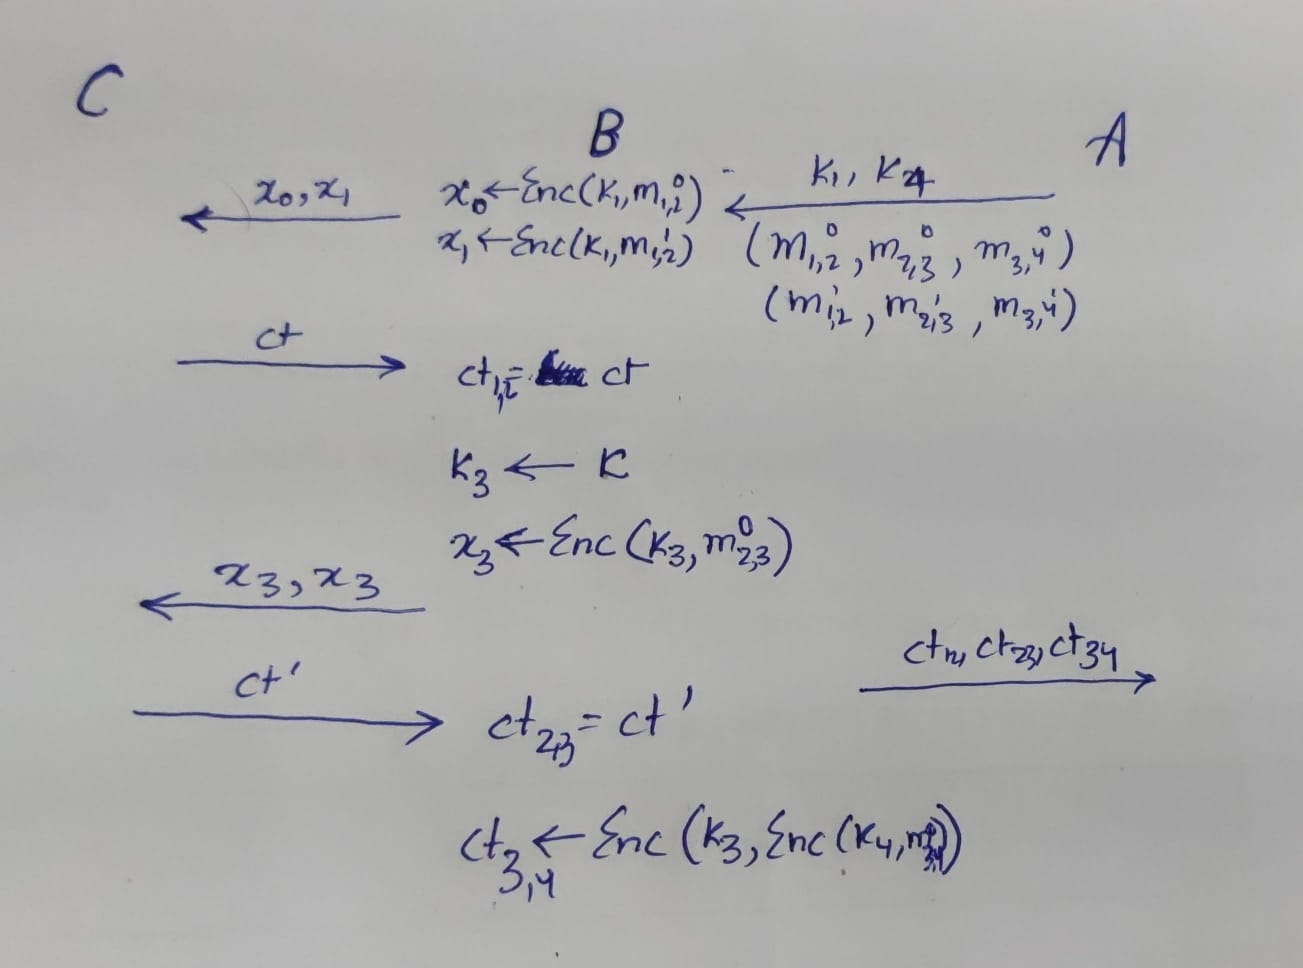
\includegraphics[scale=0.25]{images/Reduction21.jpg}
        \caption{Reduction 1 for Problem 2}
        \label{fig:p21}
    \end{figure}


    \clearpage

    \noindent\textbf{Claim:} If there exists an adversary $\calA$ for which $|p_{\hyb,0}-p_{\hyb,1}|$ is non-negligible then there exists an adversary $\calB$ which breaks the CPA security of $\calE=(\enc,\dec)$ with advantage $|p_{\hyb,0}-p_{\hyb,1}|$


    Consider the reduction \cref{red:p22}:
    \securitygame{Reduction}{Reduction 2 for Problem 2}{\label{red:p22}}
    {
        \begin{itemize}
            \item $\calA$ sends $k_1, k_4$, as well as challenge messages $(m^0_{1,2}, m^0_{2,3},m^0_{3,4})$ and $(m^1_{1,2}, m^1_{2,3},m^1_{3,4})$ to $\calB$
            \item $\calB$ samples $k_2\gets\calK$ and computes $\ct_{1,2}\gets\enc(k_2,\enc(k_1,m^1_{1,2}))$.
            \item $\calB$ sends $m^0_{2,3}, m^1_{2,3}$ to $\calC$ to obtain $\ct=\enc(k_3,m_{2,3}^b)$ and sets $\ct_{2,3}\gets\enc(k_2,\ct)$
            \item $\calB$ computes $x_0\gets\enc(k_4,m_{3,4}^0)$ and sends $(x_0,x_0)$ to $\calC$ to obtain $\ct' = \enc(k_3,\enc(k_4,m^0_{3,4}))$. $\calB$ sets $\ct_{3,4}=\ct'$
            \item $\calB$ sends $(\ct_{1,2}, \ct_{2,3}, \ct_{3,4})$ to $\calA$
            \item For the encryption queries, $\calB$ follows a similar procedure as above.
            \item Finally $\calA$ outputs a bit $b'$ which $\calB$ forwards to $\calC$
        \end{itemize}
    }

    If $\calC$ chooses $b$ to be 0 then the above reduction corresponds to Hybrid World 0  while if he chooses 1, then it corresponds to Hybrid World 1. So the CPA advantage of $\calB=|p_{\hyb,0}-p_{\hyb,1}|$
    \begin{figure}[!ht]
        \centering
        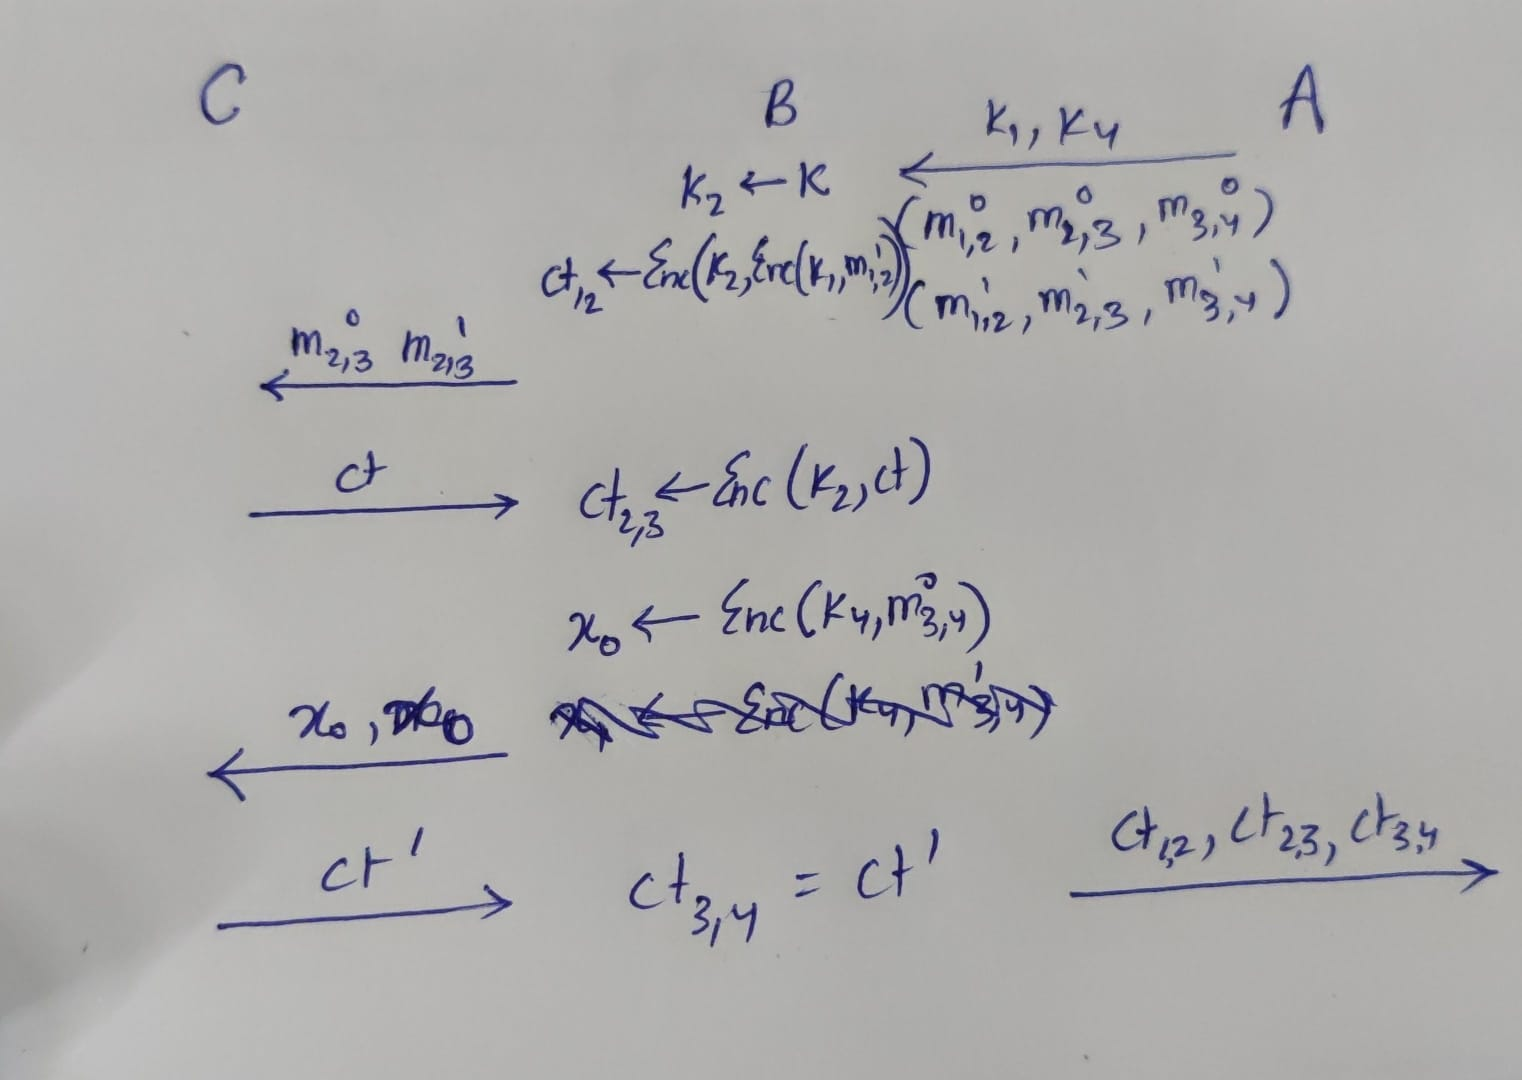
\includegraphics[scale=0.25]{images/Reduction22.jpg}
        \caption{Reduction 2 for Problem 2}
        \label{fig:p22}
    \end{figure}

    \clearpage

    \noindent\textbf{Claim:} If there exists an adversary $\calA$ for which $|p_{\hyb,1}-p_1|$ is non-negligible then there exists an adversary $\calB$ which breaks the CPA security of $\calE=(\enc,\dec)$ with advantage $|p_{\hyb,1}-p_1|$


    Consider the reduction:
    \securitygame{Reduction}{Reduction 3 for Problem 2}{\label{red:p23}}
    {
        \begin{itemize}
            \item $\calA$ sends $k_1, k_4$, as well as challenge messages $(m^0_{1,2}, m^0_{2,3},m^0_{3,4})$ and $(m^1_{1,2}, m^1_{2,3},m^1_{3,4})$ to $\calB$
            \item $\calB$ samples $k_2\gets\calK$ and computes $\ct_{1,2}\gets\enc(k_2,\enc(k_1,m^1_{1,2}))$.
            \item $\calB$ sends $m^1_{2,3}, m^1_{2,3}$ to $\calC$ to obtain $\ct=\enc(k_3,m_{2,3}^1)$ and sets $\ct_{2,3}\gets\enc(k_2,\ct)$
            \item $\calB$ computes $x_0\gets\enc(k_4,m_{3,4}^0), x_1\gets\enc(k_4,m_{3,4}^1)$ and sends $(x_0,x_1)$ to $\calC$ to obtain $\ct' = \enc(k_3,\enc(k_4,m^b_{3,4}))$. $\calB$ sets $\ct_{3,4}=\ct'$
            \item $\calB$ sends $(\ct_{1,2}, \ct_{2,3}, \ct_{3,4})$ to $\calA$
            \item For the encryption queries, $\calB$ follows a similar procedure as above.
            \item Finally $\calA$ outputs a bit $b'$ which $\calB$ forwards to $\calC$
        \end{itemize}
    }

    If $\calC$ chooses $b$ to be 0 then the above reduction corresponds to Hybrid World 1  while if he chooses 1, then it corresponds to World 1. So the CPA advantage of $\calB=|p_{\hyb,1}-p_{1}|$

    \begin{figure}[!ht]
        \centering
        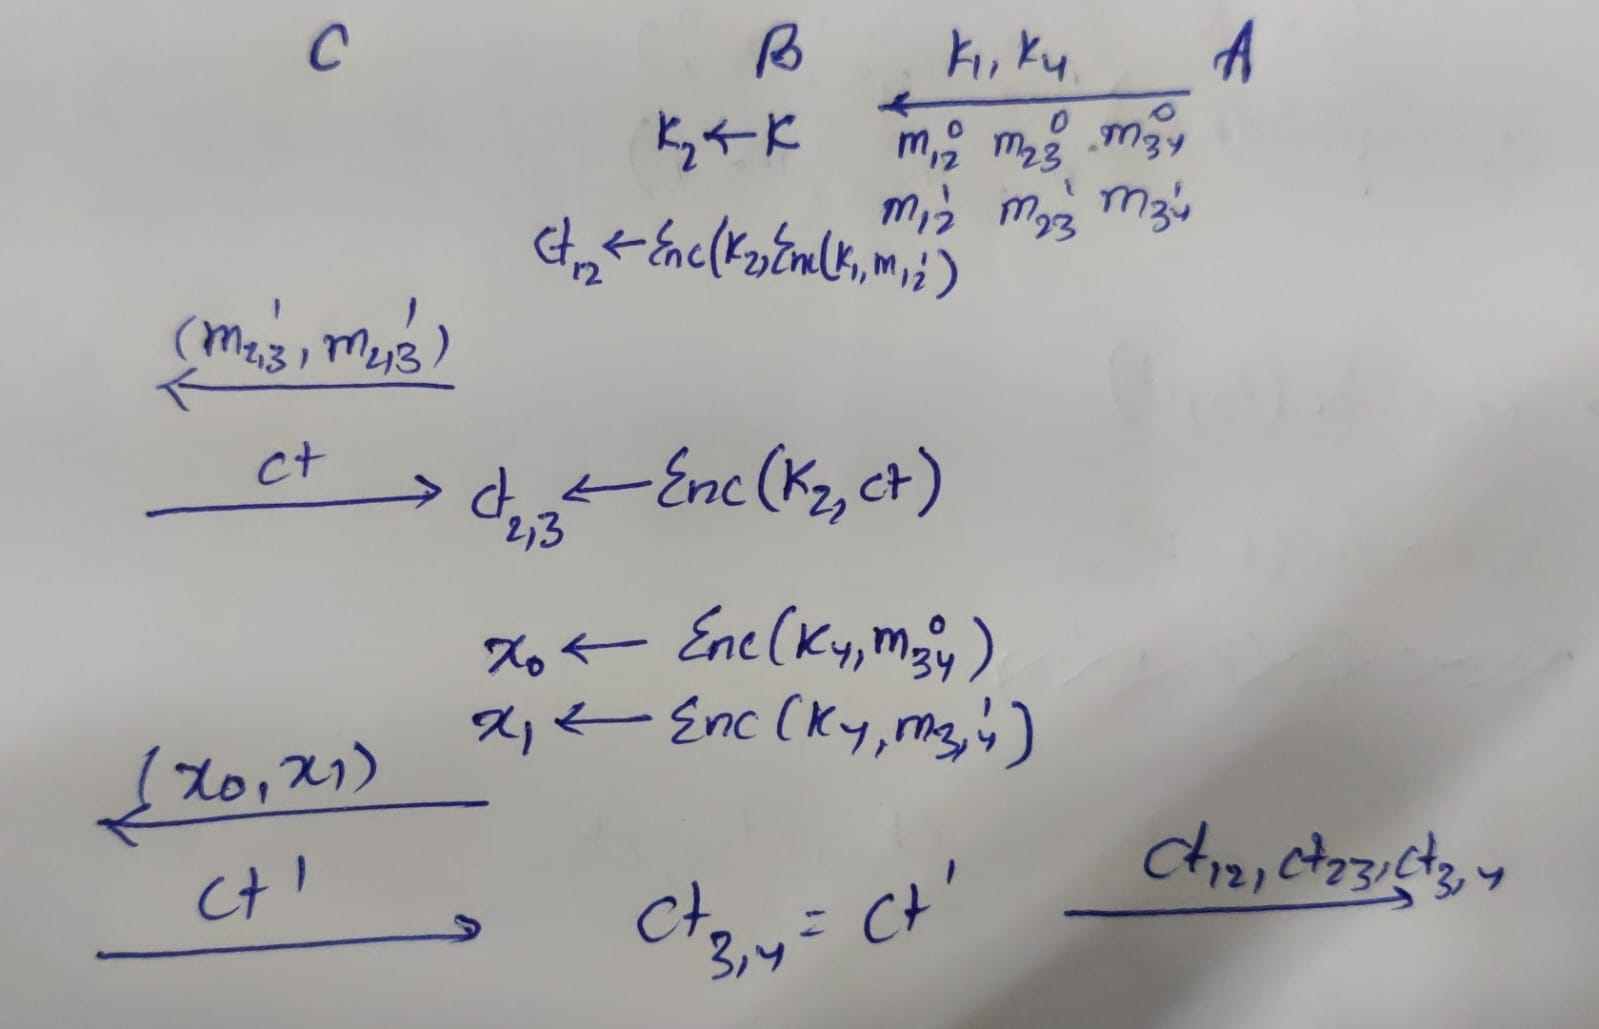
\includegraphics[scale=0.25]{images/Reduction23.jpg}
        \caption{Reduction 3 for Problem 2}
        \label{fig:p23}
    \end{figure}

    Thus from the above three claims, we can conclude that if $(\enc,\dec)$ is CPA secure, then no p.p.t. adversary has non-negligible advantage in the security game defined above.
\end{solution}

\prob{3 : One-time secure MACs, and Upgrading One-Time MACs to Many-Time MACs}
\begin{solution}

\end{solution}


\prob{4 : CCA Security v/s Authenticated Encryption}
\begin{solution}
    \begin{enumerate}[(a)]
        \item Here we need to show that CCA+PT-INT $\implies$ CT-INT. Intuitively, this is true because if an adversary breaks CT-INT, he produces a ciphertext of (1) a previously queried message or (2) a new message. If (1) happens then CCA breaks and if (2) happens then PT-INT breaks.

              Let $\calE=(\enc,\dec)$ be an encryption scheme that follows CCA and PT-INT. We will show that it satisfies CT-INT. Consider the following worlds:
              \begin{world}[World 0:]
                  This is the CT-INT game
              \end{world}

              \begin{world}[Hybrid Word]
                  This is the CT-INT game but the $\ct^*$ given as output by the adversary decrupts to one of the previously queried messages: $\dec(k,ct^*)\notin\{m_i\}$
              \end{world}

              Let $p_0$ and $p_\hyb$ be the winning probabilities of the adversary in World 0 and Hybrid World respectively.

              \textbf{Claim:} If there exists an adversary for which $|p_0-p_\hyb|$ is non-negligible then there exists a reduction $\calB$ which breaks the PT-INT of $\calE$
              \begin{proof}
                  Indeed, if $p_0$ and $p_\hyb$ are far apart then the probability that the output $\ct^*$ given by $\calA$ decrypts to a message different from the queried messages is non-negligible. The reduction simply forwards $\ct^*$ to the PT-INT challenger and wins with probability $|p_0-p_\hyb|$
              \end{proof}

              \textbf{Claim:} If there exists an adversary for which $p_\hyb$ is non-negligible then there exists a reduction $\calB$ which breaks the CCA security of $\calE$
              \begin{proof}
                  Consider the following reduction:
                  \securitygame{Reduction}{Reduction for Problem 4a}{\label{red:p4a}}
                  {
                      \begin{itemize}
                          \item $\calA$ sends $m_i$ to $\calB$
                          \item $\calB$ samples $m\gets\calM$ and sends encryption query $(m_i,m)$ to CCA challenger $\calC$
                          \item $\calC$ replies with $\ct_i$ which $\calB$ forwards to $\calA$
                          \item Finally, $\calA$ outputs $\ct^*$ which $\calB$ forwards to $\calC$ for decryption. If the output is $\perp$, $\calB$ outputs 1 otherwise it outputs 0
                      \end{itemize}
                  }
                  Let the number of queries made by $\calA$ be $Q$ and the message space be $\calM$.

                  Now, if the challenger chooses $b=0$ then it is the same as the CT-INT game.  $$\Pr[b'=0|b=0]=p_\hyb$$
                  If challenger choose $b=1$ then for all its queries, $\calA$ gets the encryption of a random message $m$. The probability of outputing 0 here will be bounded by the probability that $m\in\{m_i\}$ which is
                  $$\Pr[\exists m_i : m=m_i]\leq\frac{Q}{|\calM|}$$
                  Thus, $$\Pr[b'=0|b=1]\leq \frac{Q}{|\calM|}$$
                  $$\mathsf{CCAAdv}[\calB, \calC]\geq p_\hyb-\frac{Q}{|\calM|}$$
                  Which is non-negligible assuming $\calM$ to be superpolynomial.
              \end{proof}
        \item 
    \end{enumerate}

\end{solution}

\prob{5: Modular Arithmetic and Basic Group Theory}
\begin{solution}
    \begin{enumerate}[(a)]
        \item Since $a$ and $p$ are coprime, by the Extended Euclid's Agorithm:
              $$ ab+py=\gcd(a,p)=1    $$
              Taking modulo p on both sides:
              $$ ab \mod p =1    $$
              Where $b\in\Z_p$ (If not then by the division algorithm $b=qp+b', b'<p$. So, we can replace $b$ with $b'$)
              \vspace{20pt}

              Now suppose there exist $b, b'\in\Z_p$ such that
              $$ ab=1\mod p \hspace{50pt} ab'=1\mod p    $$
              Then by definition of mod, $p|a(b-b')$. So $b-b'=0$ since $a$ and $b-b'$ will be coprime to $p$. Hence $b$ is unique.

        \item Consider $h(y)=y^2+y$ and $n=6$. For 3 values of $y$ viz. $2,3,5$, we have $h(y)=0\mod 6$. Thus
              $$|\{y\in\Z_6:y^2+y=0\mod6\}|=3>2$$

        \item For this part, we will use Fermat's Little Theorem.
              \begin{theorem}[Fermat's Little Theorem]
                  For any prime number $p$ and $a\in\Z$
                  $$a^{p-1}=1\mod p$$
              \end{theorem}
              \begin{proof}
                  We use the following observation:

                  \textbf{Observation:} Let $a \in\Z^*_p$. Consider the set $S_a = \{a\cdot i: i\in\Z^*_p\}$. Then $S_a = \Z^*_p$.

                  Otherwise, suppose there exist $i,j\in\Z^*_p$ such that $$a\cdot i \mod p= a\cdot j\mod p\implies p | a (i-j)\implies i=j$$

                  Now consider the product of all elements of $S_a$

                  $$\prod_{a_i\in S_a}a_i=\prod_{i=1}^{p-1}a\cdot i=a^{p-1}\prod_{i\in\Z^*_p}i$$
                  Since $S_a = \Z^*_p$, the products on both sides must be the same. Hence $$a^{p-1}=1\mod p$$


              \end{proof}
              Let $a\in\Z_p$ and $r=\ord(a)$. Then $a^r=1\mod p$. By Fermat's Little Theorem:
              $$a^{p-1}=1\mod p$$
              Suppose by the division algorithm, $p-1=rq+s$, $s<r$. Since $a^{p-1}=1\mod p$ and $a^{r}=1\mod p$, $$a^{p-1-rq}=1\mod p$$ and hence $a^{s}=1\mod p$. But since $s<r$, $s$ must be 0.

        \item Observe that the given distribution $\calD_0$ is a modification of the $\ddh$ distibution $$\calD'_0=\{(g, g^a, g^b, g^{a\cdot b}) : g\gets G, a,b\gets\Z^*_p \}$$ where $b=a^2$. So, an Adversary which can distinguish between $\calD'_0$ and $\calD_1$ should also be able to distinguish between $\calD_0$ and $\calD_1$.

              The reduction $\calB$ simply forwards the message it receives from the challenger to $\calA$ and forwards the output of $\calA$ to $\calC$ as showin in \cref{fig:p5d}
              \begin{figure}[!ht]
                  \centering
                  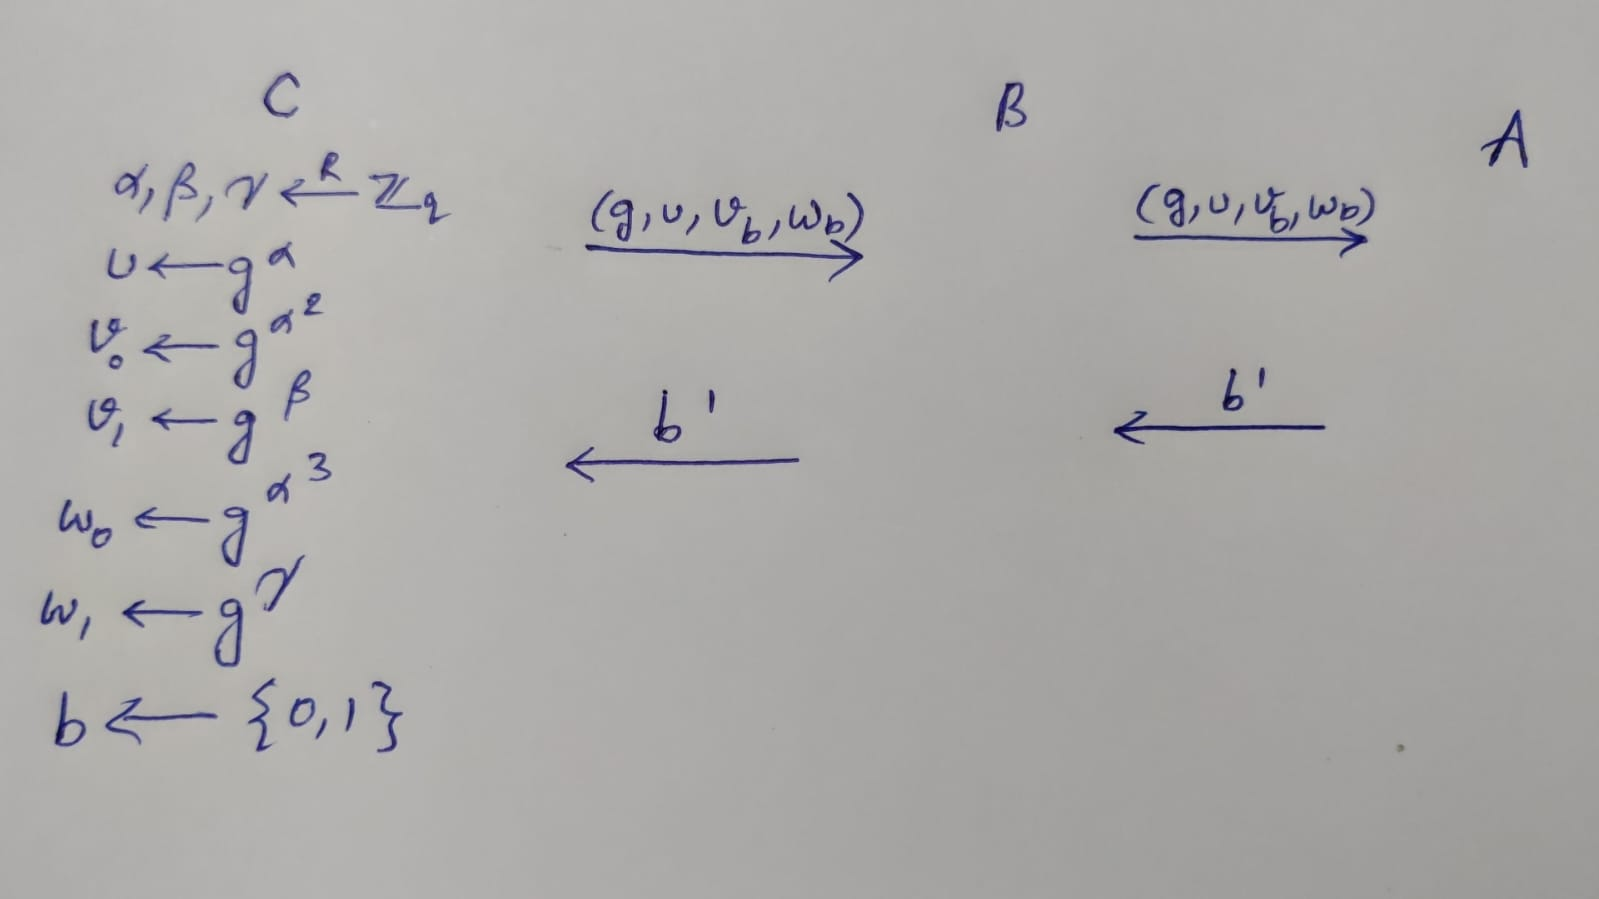
\includegraphics[scale=0.25]{images/Reduction5d.jpg}
                  \caption{Reduction for Problem 5d}
                  \label{fig:p5d}
              \end{figure}

        \item Let $S_i$ denote the set of matrices $M\in\Z_q^{t\times t}$ where the last $i$ rows are of the form
              $$\lambda_j (v_1 \dots v_t),\hspace{20pt} j\in[i], (v_1 \dots v_t)\gets\Z_q^t, \lambda_j\gets\Z_q$$

              and the remaining rows have elements sampled at random from $\Z_q$. In other words, last $i$ rows are random multiples of some tuple (chosen at random) and remaining rows are drawn at random. Observe that $S_n=\mathsf{Rank}_1[t,q]$ and $S_1=\Z_q^{t\times t}$.

              The proof proceedes by a sequence of $n$ hybrid worlds:
              \begin{world}[Hybrid World $\mathbf{i}$:]
                  The Challenger samples from the distribution $$\calD'_i=\{(g,g^\mathbf{M}): g\gets G,\mathbf{M}\gets S_i \}$$
              \end{world}
              Observe that Hybrid World 1 corresponds to sampling from $\calD_1$ and Hybrid World $n$ corresponds to sampling from  $\calD_0$ specified in the question.
              Let $p_i$ be the probability of the Adversary outputting 0 in the above Hybrids.

              \textbf{Claim:} If there exists an adversary $\calA$ such that $|p_i-p_{i+1}|$ is non-negligible then there exists an adversary $\calB$ which solves the DDH problem for group $G$.

              \begin{proof}
                  Consider the following reduction:


                  \securitygame{Reduction}{Reduction for Problem 5e}{\label{red:p5e}}
                  {
                      \begin{itemize}
                          \item $\calC$ samples $b\gets\bit$ and $g\gets G$. He calculates $g^\alpha, g^\beta$ and $w_0=g^{\alpha\cdot\beta}, w_1=g^\gamma$ where $\alpha,\beta,\gamma\gets\Z_q$ and sends $(g, g^\alpha, g^\beta, w_b)$ th $\calB$
                          \item $\calB$ samples the following:
                                $$\beta_1,\beta_2,\dots\beta_{t-1}\gets\Z_q$$
                                $$\lambda_1,\lambda_2,\dots\lambda_{i}\gets\Z_q$$
                                $$v_{i,j}\gets\Z_q\hspace{20pt}1\leq i\leq {t-i-1}, 1\leq j \leq t$$
                                And computes the matrix:
                                $$
                                    \begin{bmatrix}
                                        g^{v_{1,1}}        & g^{v_{1,2}}          & \dots  & g^{v_{1,t}}              \\
                                        \vdots             & \vdots               & \ddots & \vdots                   \\
                                        g^{v_{t-i-1,1}}    & g^{v_{t-i-1,2}}      & \dots  & g^{v_{t-i-1,t}}          \\
                                        w_b                & g^{\alpha\beta_1}    & \dots  & g^{\alpha\beta_{t-1}}    \\
                                        g^{\lambda_i\beta} & g^{\lambda_i\beta_1} & \dots  & g^{\lambda_i\beta_{t-1}} \\
                                        \vdots             & \vdots               & \ddots & \vdots                   \\
                                        g^{\lambda_1\beta} & g^{\lambda_1\beta_1} & \dots  & g^{\lambda_1\beta_{t-1}}
                                    \end{bmatrix}
                                $$
                                And sends it to $\calA$

                          \item $\calA$ responds with a bit $b'$ which $\calB$ forwards to $\calC$
                      \end{itemize}
                  }

                  \begin{figure}[!ht]
                      \centering
                      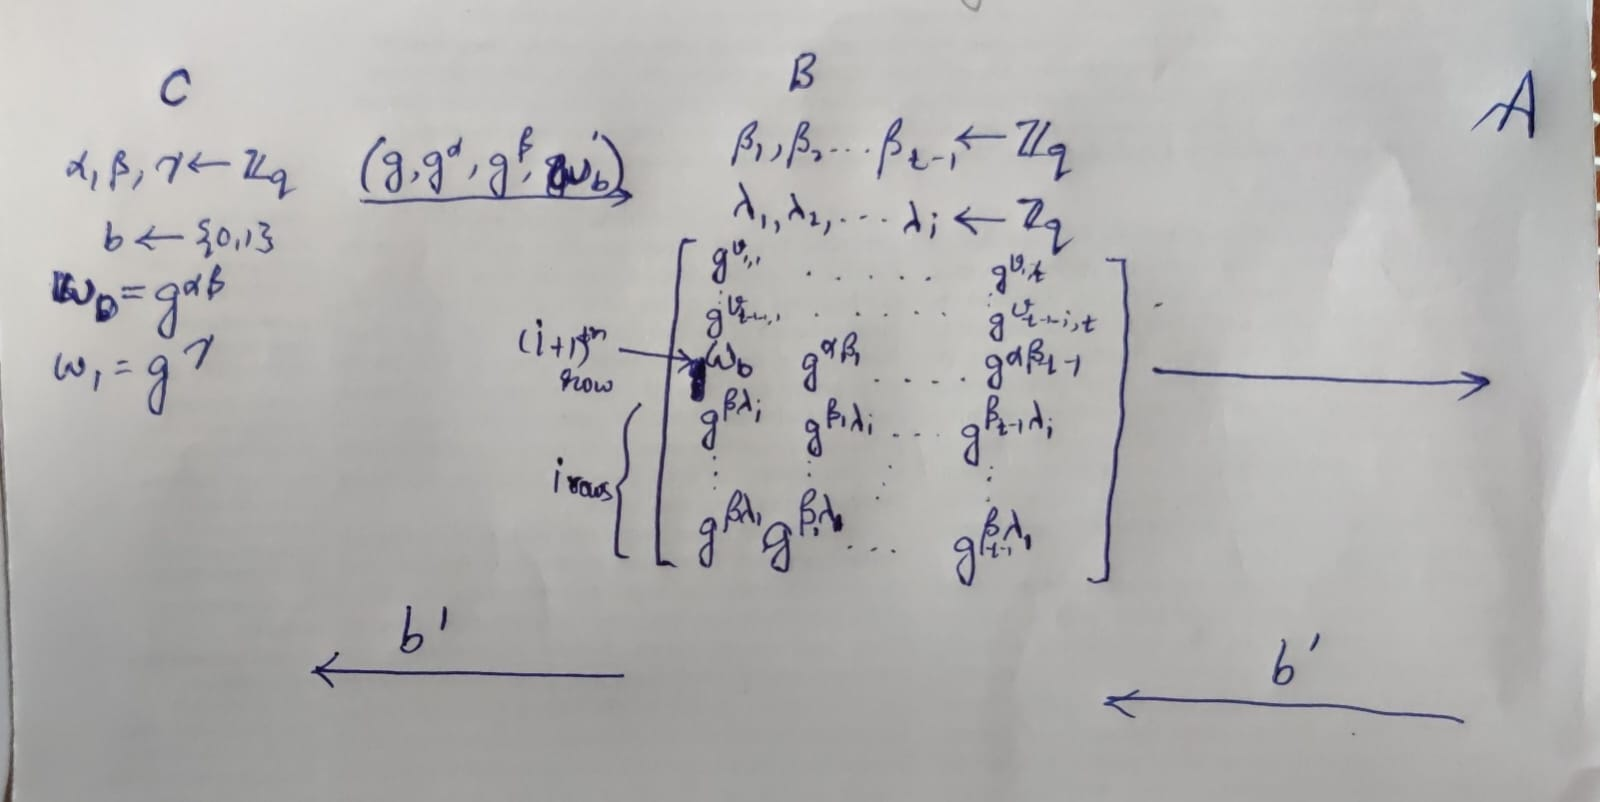
\includegraphics[scale=0.25]{images/Reduction5e.jpg}
                      \caption{Reduction for Problem 5e}
                      \label{fig:p5e}
                  \end{figure}

                  Observe that if $b=0$ then it corresponds to Hybrid World $i+1$ and if $b=1$ then it corresponds to Hybrid World $i$. This is because the matrix
                  $$
                      \begin{bmatrix}
                          {v_{1,1}}        & {v_{1,2}}          & \dots  & {v_{1,t}}              \\
                          \vdots           & \vdots             & \ddots & \vdots                 \\
                          {v_{t-i-1,1}}    & {v_{t-i-1,2}}      & \dots  & {v_{t-i-1,t}}          \\
                          \alpha\beta      & {\alpha\beta_1}    & \dots  & {\alpha\beta_{t-1}}    \\
                          {\lambda_i\beta} & {\lambda_i\beta_1} & \dots  & {\lambda_i\beta_{t-1}} \\
                          \vdots           & \vdots             & \ddots & \vdots                 \\
                          {\lambda_1\beta} & {\lambda_1\beta_1} & \dots  & {\lambda_1\beta_{t-1}}
                      \end{bmatrix}
                  $$
                  Has the last $i+1$ rows as the multiple of the tuple $(\beta, \beta_1, \beta_2\dots\beta_{t-1})$ while
                  $$
                      \begin{bmatrix}
                          {v_{1,1}}        & {v_{1,2}}          & \dots  & {v_{1,t}}              \\
                          \vdots           & \vdots             & \ddots & \vdots                 \\
                          {v_{t-i-1,1}}    & {v_{t-i-1,2}}      & \dots  & {v_{t-i-1,t}}          \\
                          \gamma           & {\alpha\beta_1}    & \dots  & {\alpha\beta_{t-1}}    \\
                          {\lambda_i\beta} & {\lambda_i\beta_1} & \dots  & {\lambda_i\beta_{t-1}} \\
                          \vdots           & \vdots             & \ddots & \vdots                 \\
                          {\lambda_1\beta} & {\lambda_1\beta_1} & \dots  & {\lambda_1\beta_{t-1}}
                      \end{bmatrix}
                  $$
                  Has the last $i$ rows as the multiple of the tuple $(\beta, \beta_1, \beta_2\dots\beta_{t-1})$. Hence, $$\mathsf{DDHAdv}[\calB, \calC]=|p_i-p_{i+1}|$$
              \end{proof}
              \vspace{20pt}
              Therefore we observe that the hybrid worlds are computationally indistinguishable. Assuming that the DDH problem is hard on $G$,
              $$|p_1-p_{n}|\leq \sum_{i=1}^{n-1}|p_i-p_{i+1}|$$
              Which is negligible assuming $|p_i-p_{i+1}|$ is negligible. So, $\calD_0$ and $\calD_1$ are computationally indistinguishable.



    \end{enumerate}
\end{solution}

\end{document}
